Das Backend soll wie in Kapitel 2.3 beschrieben die Datenquelle f�r die
verschiedenen Clients sein. Umgesetzt werden soll dies �ber einen RESTful
Service. Es wird das Framework "`Spring"' eingesetzt. Dies erlaubt eine einfache
Erstellung von Web-Services und unterst�tzt den Programmierer mit Werkzeugen wie
Hibernate, die die Verwaltung der Datenbank stark vereinfacht und �nderungen an
der Modellierung direkt in der Datenbank umsetzt.
\subsection{Anforderungen}
Das Backend soll den Clients die Daten wie oben genannt �ber einen
RESTful-Service zur Verf�gung stellen. Dies vereinfacht den Zugriff auf die
Ressourcen und ist leicht in bestehende Infrastrukturen einzubinden. Das Backend
soll nach M�glichkeit �ber \ac{https} zur Verf�gung stellen, damit �bertragene
Daten auf dem Weg gesichert sind. Eine Authentifizierung auf Zugriffsebene ist
optional, da der Service in einem geschlossenen Netz betrieben werden soll. Das
Backend soll zudem Authentifizierungsanfragen auf Anwendungsebene bearbeiten. 
\subsection{Implementierung}
	Das Backend wird mit dem quelloffenen Framework Spring umgesetzt. Spring bietet
	wie in Kapitel \ref{Spring} auf Seite \pageref{Spring} beschrieben Funktionen
	wie Dependency Injection und �hnliches, das die Implementierung eines
	Webservices erheblich vereinfacht. Die f�r dieses Projekt verwendeten Module
	umfassen Spring Boot und Spring Data. Spring Boot erlaubt die einfache
	Erstellung sofort lauff�higer Spring-Anwendungen, da hier keine komplexen
	XML-Konfigurationen vorgenommen werden m�ssen, und das Projekt �bersichtlich
	genug, um keine komplexen Konfigurationen zu ben�tigen.
	\subsubsection{Datenbank}
		Die Datenbank wird von Hibernate (Siehe Kapitel \ref{Hibernate}, Seite
		\pageref{Hibernate}) aus dem Objektmodell generiert. Hierzu werden die
		Tabellennamen, Beziehungen und die Optionen wie zum Beispiel "`Not Null"'
		mithilfe von Annotationen an Hibernate weitergegeben. Aus diesen Informationen
		erstellt Hibernate das relationale Datenmodell(Siehe Abbildung
		\ref{fig:er_model}, Seite \pageref{fig:er_model}).
	 \begin{figure}[H]
		\begin{minipage}{\linewidth}
		 	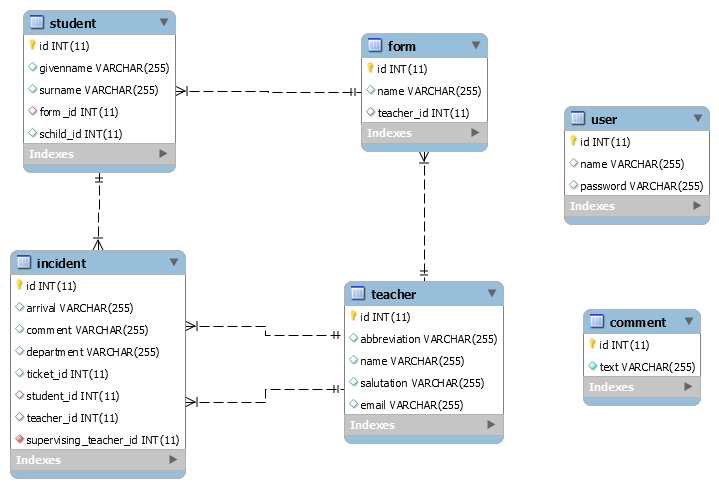
\includegraphics[width=0.9\linewidth]{grafx/ER_Model}
 			\caption[ER-Modell der Datenbank]{ER-Modell der Datenbank}
  			\label{fig:er_model}
		\end{minipage}
	\end{figure}
	\begin{description}
	\item[teacher]
		Die "`teacher"'-Tabelle h�lt Daten �ber die Lehrer vor. Dies umfasst den
		vollen Namen (name), die Abk�rzung (abbreviation) und die Anrede (salutation)
	\item[form]
		Die "`form"'-Tabelle h�lt Daten �ber die Schulklassen vor, dies beinhaltet die
		Bezeichnung der Klasse (name) und einen Fremdschl�ssel "`teacher\_id"', der
		den Klassenlehrer referenziert.
	\item[student]
		Die "`student"'-Tabelle h�lt Daten �ber die Sch�ler, die im System erfasst
		sind, vor. Dies umfasst den Namen des Sch�lers geteilt in Vor- und Nachname
		(givenname, surname) und einen Fremdschl�ssel "`form\_id"', die die
		Schulklasse, der der Sch�ler angeh�rt referenziert. Zudem wird die
		Identifikationsnummer des Sch�lers gespeichert, um gleichnamige Sch�ler
		eindeutig identifizieren zu k�nnen (schild\_id).
	\item[incident]
		In der "`incident"'-Tabelle werden alle Vorf�lle gespeichert, die �ber den
		TRManager eingetragen werden. Dazu geh�ren die Ankunftszeit (arrival), der
		Zeitpunkt der "`Entlassung"' (department), den zugeh�rigen Sch�ler (\ac{FK}
		student\_id), den schickenden Lehrer (\ac{FK} teacher\_id), ein Kommentarfeld
		(comment) und eine interne Vorfallsnummer, die Ticket ID(ticket\_id).
	\end{description}

\subsection{Tests }


	\subsubsection{In Memory DB ?}


\subsection{Generischer Controller ??}
 